\documentclass[a4paper,14pt]{extarticle}
\usepackage{../../tex-shared/report-layout}

\renewcommand{\mylabnumber}{2}
\renewcommand{\mylabtitle}{Сравнение итерационного и рекурсивного методов решения задач}
\renewcommand{\mysubject}{Методы и средства искусственного интеллекта}
\renewcommand{\mylecturer}{Сметанина Т.И.}

\begin{document}
\begin{titlepage}
    
    \thispagestyle{empty}
    
    \begin{center}
        
        Министерство науки и Высшего образования Российской Федерации \\
        Севастопольский государственный университет \\
        Кафедра ИС
        
        \vfill

        Отчет \\
        по лабораторной работе №\mylabnumber \\
        \enquote{\mylabtitle} \\
        по дисциплине \\
        \enquote{\MakeTextUppercase{\mysubject}}

    \end{center}

    \vspace{1cm}

    \noindent\hspace{7.5cm} Выполнил студент группы ИС/б-17-2-о \\
    \null\hspace{7.5cm} Горбенко К. Н. \\
    \null\hspace{7.5cm} Проверил \\
    \null\hspace{7.5cm} \mylecturer

    \vfill

    \begin{center}
        Севастополь \\
        \the\year{}
    \end{center}

\end{titlepage}

\section{Цель работы}
Исследование способов организации циклических вычислений в языке Лисп с помощью
итерационного и рекурсивного методов, сравнение указанных методов по
вычислительной эффективности и выразительности, получение практических навыков
работы со списочными структурами.

\section{Задание на работу}
Задача: описать функцию, которая добавляет число в упорядоченный по возрастанию
список без нарушения порядка рекурсивно и с помощью механизмов организации
итерационных циклов. Сравнить оба способа по вычислительной эффективности.
Рекурсивное решение должно удовлетворять требованиям функционального
программирования.

\section{Ход работы}
Составим функцию для решения задачи рекурсивно.

\begin{lstlisting}
(defun addToSortedListRecursive (item list)
  (if (null list)
    (list item)
    (if (> item (first list))
      (append (list (first list)) (addToSortedListRecursive item (cdr list)))
      (append (list item) list)
    )
  )
)
\end{lstlisting}

В данном листинге использованы следующие функции:
\begin{itemize}
    \item \code{null} -- для проверки массива на \code{NIL}.
    \item \code{append} -- объединяет несколько списков в один.
\end{itemize}

Для сравнения приведу функцию, выполняющую те же функции на языке \code{F\#}
(также функциональном).

\begin{lstlisting}
let rec addToSortedListRecursive item list =
    match list with
    | [] -> [ item ]
    | head :: tail -> if item > head
                        then head :: (addToSortedListRecursive item tail)
                        else item :: list
\end{lstlisting}

На мой взгляд, функциональный подход в языке \code{LISP} менее выразителен, чем
в современных функциональных языках программирования.

Функция для итерационного вычисления:

\begin{lstlisting}
(defun getRange (list start end)
  (loop for i from start to end
    collect (nth i list)
  )
)

(defun range (min max step)
  (loop for n from min below max by step
    collect n
  )
)

(defun addToSortedListIterative (item list)
  (cond
    ((null list) (list item))
    ((> item (car (last list))) (append list (list item)))
    ((< item (first list)) (append (list item) list))
    (T (loop for i in (reverse (range 0 (length list) 1))
      when (> item (nth i list))
        return (append (getRange list 0 i) (list item) (getRange list (+ i 1) (- (length list) 1)))
    ))
  )
)
\end{lstlisting}

В функции \code{addToSortedListIterative} перед проведением итерации происходит
проверка пограничных случаев (список пуст, вставляемый элемент -- первый или
последний в результирующем списке). Затем при итерации последовательно находим
позицию, в которую нужно вставить элемент и формируем новый список.

Использованные функции:
\begin{itemize}
    \item \code{loop} -- макро для организации циклов.
    \item \code{reverse} -- оборачивает список.
    \item \code{return} -- возвращает результат из цикла (функции \code{loop}).
    \item \code{length} -- возвращает размер списка. 
\end{itemize}

Составим тестовые случаи:

\begin{lstlisting}
(print (addToSortedListRecursive 15 nil))
(print (addToSortedListRecursive 15 (list 3)))
(print (addToSortedListRecursive -15 (list 3)))
(print (addToSortedListRecursive 15 (list 1 2 3)))
(print (addToSortedListRecursive -15 (list 1 2 3)))
(print (addToSortedListRecursive 3 (list 1 2 15)))

(print (addToSortedListIterative 15 nil))
(print (addToSortedListIterative 15 (list 3)))
(print (addToSortedListIterative -15 (list 3)))
(print (addToSortedListIterative 15 (list 1 2 3)))
(print (addToSortedListIterative -15 (list 1 2 3)))
(print (addToSortedListIterative 3 (list 1 2 15)))
\end{lstlisting}

Результат выполнения программы изображен на рисунке \ref{fig:result}:

\begin{figure}[H]
    \centering
    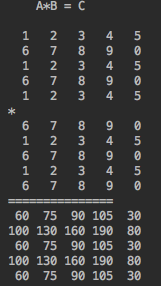
\includegraphics[width=.7\linewidth]{result}
    \caption{Результат выполения программы}
    \label{fig:result}
\end{figure}

По рисунку \ref{fig:result} видно, что две функции работают одинаково.

\section*{ВЫВОДЫ}
В ходе лабораторной работы были исследованы рекурсивный и итерационный подходы
языка программирования \code{LISP}. Для решения задачи были разработаны две
функции с помощью разных подходов. Рекурсивная функция значительно компактнее и
проще, чем итерационная. Кроме того, на мой взгляд, она более выразительна.

Тем не менее, рекурсивная функция менее выразительна, чем такая же на
современном языке.

\end{document}